
\documentclass[12pt]{article}
%%%%%%%%%%%%%%%%%%%%%%%%%%%%%%%%%%%%%%%%%%%%%%%%%%%%%%%%%%%%%%%%%%%%%%%%%%%%%%%%%%%%%%%%%%%%%%%%%%%%%%%%%%%%%%%%%%%%%%%%%%%%%%%%%%%%%%%%%%%%%%%%%%%%%%%%%%%%%%%%%%%%%%%%%%%%%%%%%%%%%%%%%%%%%%%%%%%%%%%%%%%%%%%%%%%%%%%%%%%%%%%%%%%%%%%%%%%%%%%%%%%%%%%%%%%%
\usepackage{amssymb}
\usepackage{amsmath}
\usepackage{graphicx}
\usepackage{chicago}
\usepackage{rotating}
\usepackage{hyperref}
\usepackage{sectsty}




\setcounter{MaxMatrixCols}{10}
%TCIDATA{OutputFilter=Latex.dll}
%TCIDATA{Version=5.50.0.2960}
%TCIDATA{<META NAME="SaveForMode" CONTENT="1">}
%TCIDATA{BibliographyScheme=Manual}
%TCIDATA{LastRevised=Tuesday, June 18, 2013 11:50:19}
%TCIDATA{<META NAME="GraphicsSave" CONTENT="32">}

\setlength{\paperwidth}{8.5in} \setlength{\paperheight}{11.0in}
\setlength{\topmargin}{0.0in} \setlength{\headheight}{0.4in}
\setlength{\headsep}{0.0in} \setlength{\textwidth}{7.2in}
\setlength{\textheight}{8.5in} \setlength{\oddsidemargin}{0.0in}
\setlength{\oddsidemargin}{-0.4in}
\setlength{\evensidemargin}{-0.4in}
\newtheorem{theorem}{Theorem}
\newtheorem{acknowledgement}[theorem]{Acknowledgement}
\newtheorem{algorithm}[theorem]{Algorithm}
\newtheorem{axiom}[theorem]{Axiom}
\newtheorem{case}[theorem]{Case}
\newtheorem{claim}[theorem]{Claim}
\newtheorem{conclusion}[theorem]{Conclusion}
\newtheorem{condition}[theorem]{Condition}
\newtheorem{conjecture}[theorem]{Conjecture}
\newtheorem{corollary}[theorem]{Corollary}
\newtheorem{criterion}[theorem]{Criterion}
\newtheorem{definition}[theorem]{Definition}
\newtheorem{example}[theorem]{Example}
\newtheorem{exercise}[theorem]{Exercise}
\newtheorem{lemma}[theorem]{Lemma}
\newtheorem{notation}[theorem]{Notation}
\newtheorem{problem}[theorem]{Problem}
\newtheorem{proposition}[theorem]{Proposition}
\newtheorem{remark}[theorem]{Remark}
\newtheorem{solution}[theorem]{Solution}
\newtheorem{summary}[theorem]{Summary}
\newenvironment{proof}[1][Proof]{\noindent\textbf{#1.} }{\ \rule{0.5em}{0.5em}}
\input{tcilatex}
\renewcommand{\baselinestretch}{1.5}
\renewcommand{\textfraction}{0.33}

\begin{document}


\bigskip

\bigskip

\clearpage

\renewcommand{\baselinestretch}{1.0}

\begin{center}
{\normalsize \thispagestyle{empty} }

{\normalsize \medskip }

{\normalsize {\Large Forecasting Net Interest Margins of Banks$^{*}$}
\medskip }

{\normalsize \bigskip \bigskip }

{\normalsize Valentin Bolotnyy, Rochelle Edge, and Luca Guerrieri }

{\normalsize \bigskip \bigskip }

{\normalsize April 29, 2013 }

{\normalsize \bigskip }
\end{center}

{\normalsize \bigskip }

\abstract{}

{\normalsize \vspace{3.0cm} }

{\normalsize \noindent \textbf{Keywords}: \vspace{1cm} }

{\normalsize \noindent \textbf{JEL Classification}: }

{\normalsize \vspace{2cm} }

\renewcommand{\baselinestretch}{1} {\footnotesize \noindent }

{\footnotesize \textbf{\ Affiliation and contact information}: Valentin
Bolotnyy, Federal Reserve Board, telephone (202) 452-6428, email
valentin.bolotnyy@frb.gov; Rochelle Edge, Federal Reserve Board, telephone
(202) 452-2339, email rochelle.m.edge@frb.gov; Luca Guerrieri, Federal
Reserve Board, telephone (202) 452-2550, email luca.guerrieri@frb.gov. }

{\footnotesize \vspace{2cm} }

{\footnotesize \noindent $^{*}$ The views expressed in this paper are solely
the responsibility of the authors and should not be interpreted as
reflecting the views of the Board of Governors of the Federal Reserve System
or of any other person associated with the Federal Reserve System. }

{\footnotesize \clearpage \renewcommand{\baselinestretch}{1.5} }

\section{\protect\normalsize Introduction}

{\normalsize Regular bank stress testing (and the capital planning that it
implies) is one of the three complementary reforms that has been made to the
capital regulatory regime made in response to the shortcomings of the
pre-crisis system. While stress testing can take many forms - such as, being
based on a small number of scenarios, being based on a large number of
scenarios, or even being undertaken in reverse form to achieve a certain
adverse outcome - the form of stress testing mandated under the Dodd-Frank
Act for U.S. bank regulators and the form being used by the Federal Reserve
for its annual Comprehensive Capital Analysis and Review (CCAR) is one based
around small number of scenarios. This approach involves specifying a small
set of macroeconomic and financial scenarios that represents stressful
conditions over the time horizon of the stress test and then projecting, for
each BHC in the stress test, its losses, income, and path of pro-forma
capital based on the scenario. Clearly, therefore, there are at least two
important parts to conducting bank stress tests: Formulating the
macroeconomic and financial scenarios that a priori would seem stressful to
banks and developing models that are able to translate such stressful
conditions into losses, income, and pro-forma capital. This paper considers
an aspect of the latter of these two issues. In developing models to
translate stressful macroeconomic and financial conditions into bank income-
and balance-sheet variables it is useful to consider the types of
developments, and for which particular variables, that are likely to be
stressful to banks. This is because adverse developments in these variables
are very likely to be featured in one of the specified stressful scenarios.
Moreover, it is also desirable that the models being used for stress testing
are able to translate developments in these variables well into the key
income- or balance-sheet variable that the model is designed to project. In
this paper, we examine this property for models of bank net interest margins
(NIMs) defined as the ratio of net interest income (NII) to interest earning
assets, where NII is the difference between a bank's interest income and
interest expenses. Our motivation for focusing on models of NIMs is based on
a number of considerations. First, bank losses that arise from banks' having
to pay out more in interest of their liabilities than they are earning from
their assets should not be overlooked as an important source of risk to the
banking and broader financial sector. To be sure, this form of losses was
much less prominent in the most recent crisis relative to the form of bank
losses that stem from loan defaults. But, there are ample examples of other
earlier banking crises in which adverse developments in NIMs have played a
significant role. The most familiar of these from the U.S. perspective is
the Savings and Loans (S\&L) crisis of the late 1980s and early 1990s in
which - as a result of the Volcker disinflation - short-term interest rates
rose above long-term interest rates, interest expenses rose above interest
income, NII and NIMs turned negative (in the thrift sector), and sizable
losses and a substantial number of bank failures resulted. Likewise, the
three Nordic banking crises of the late 1980s and early 1990s (for Finland,
Sweden, and Norway) - which represent three out of Reinhart's and Rogoff's
(2009) "big five" banking crises - were associated with high short-term
interest rates that turned NII and NIMs negative and lead to sizable bank
losses and failures. Additionally, the U.K.'s secondary banking crisis of
the early 1970s was associated with a sudden increase in short-term interest
rates that abruptly drove up banks' costs of funds so too leading to losses
and failures. To be sure, large increases in short-term rates and declines
in net interest income were not the only reason for any of these crises but
the role of short-term interest rates - and, in particular, their elevated
level relative to long-term interest rates was material and in most cases
equivalent in importance to the other causes of the crisis. Another
motivation for our focus on models of NIM stems from the recent lackluster
pace of bank profit growth. Bank net income growth in recent years has been
largely supported by unsustainable cost cutting and reductions in
provisioning, rather than from traditional sources of bank
revenue-generation like NII. NII growth, for example, (in both nominal and
real terms) has been well below average in recent years while NIMs (NII
relative to interest earning assets) have also been low. Given their already
low level, any adverse development that puts further downward pressure on
NIMs could be very stressful for banks and, as such, it is important that
the economic developments (likely involving interest rates) that would drive
these outcomes are well-modeled. Figure 1 - Net interest income growth (LHS)
and net interest margins (RHS) }

{\normalsize Our final motivation for examining NIMs is that despite the
importance of NIMs for the financial condition of banks, the modeling of
NIMs has received much less attention in the literature relative to modeling
of bank financial-statement variables related to credit losses. To be sure,
the recent increase in the importance of stress testing has led to the
development of a number of models that link NIMs to macroecnomic variables -
such as, short-term Treasury rates and the slope of the Treasury yield curve
- where Kovner et al. (2011) and Covas et al. (2012) are notable examples.
However, this research has given relatively little attention to the
conditional forecasting properties of these models, which is important if
these models are ultimately to be used to project bank losses, income, and
pro-forma given macroeconomic scenarios. In this paper we consider a range
of different models of NIMs, developed with varying degrees of modeling
complexity, and examine how well these models explain NIMs. An important
emphasis in examining how well these models explain NIMs is
pseudo-out-of-sample forecast performance. We adopt this approach for the
simple reason that the evaluation of models based on their in-sample
forecast performance, frequently leads to the econometrician over-fitting
the model within the sample so as to maximize in-sample forecast
performance. And this leads to the model performing very poorly once it
starts to be used beyond the estimation sample. Model evaluation based on
pseudo-out-of-sample forecast performance indemnifies the econometrician
somewhat from this tendency. We also try to limit the tendency to fine-tune
the model to obtain better performing (now pseudo-out-of-sample) forecasts
by remaining fairly restrained in terms of choosing additional variables to
include in the model. For the most part we use only the most obvious
variables in our models; specifically, those that we can make a fairly
strong theoretical justification for and those that appear frequently in
other models of NIMs. We have already noted a couple of papers that attempt
to model NIMs, but there are several additional ones. OF RECENT PAPERS
SKANDER AND LISA. NOTE TWO PARTS TO THE LITERATURE OLD AND NEW AND BANKING
AND MACRO. }

\section{\protect\normalsize Models}

1. \textbf{Simple Forecast Combination}. \ We regress NIMs on each yield $r(\tau )_{t-1}$ separately: \
\begin{equation*}
NIM_{t}=c_{\tau }+\rho _{\tau }NIM_{t-1}+\gamma _{\tau }r(\tau )_{t-1}+{\eta
_{\tau ,t}}
\end{equation*}

Each regression is use to produce an $s$ step-ahead forecast of NIMs
conditional on yields on treasuries with maturity $\tau $ observed through
period $t+s-1.$ This conditional forecast is denoted by $NIM_{\tau ,t+s/t}.$%
The simple forecast comnination is then given by:%
\begin{equation*}
NIM_{t+s/t}=\sum_{\tau }\frac{NIM_{\tau ,t+s/t}}{N},
\end{equation*}%
where $N$ is the number of maturities considered.

2. \textbf{A Dynamic Factor Model for NIMs.} \ Using the state space
representation, the state equations of our restricted dynamic factor model
is given by

\begin{equation*}
\left(
\begin{array}{c}
{L_{t+1}-\mu _{L}} \\
{S_{t+1}-\mu _{S}} \\
{C_{t+1}-\mu _{C}} \\
\widehat{NIM}_{t+1}-\mu _{\widehat{NIM}}%
\end{array}%
\right) {\normalsize \ =\ }\left(
\begin{array}{cccc}
a_{11} & a_{12} & a_{13} & 0 \\
a_{21} & a_{22} & a_{23} & 0 \\
a_{31} & a_{32} & a_{33} & 0 \\
a_{41} & a_{42} & a_{43} & a_{44}%
\end{array}%
\right) {\normalsize \ }\left(
\begin{array}{c}
{L_{t}-\mu _{L}} \\
{S_{t}-\mu _{S}} \\
{C_{t}-\mu _{C}} \\
\widehat{NIM}_{t}-\mu _{\widehat{NIM}}%
\end{array}%
\right) {\normalsize +}\left(
\begin{array}{c}
{\eta _{Lt}} \\
{\eta _{St}} \\
{\eta _{Ct}} \\
{\eta _{NIMt}}%
\end{array}%
{\normalsize \ }\right) ,
\end{equation*}

where $L_{t},S_{t},$ and $C_{t}$ are level slope and curvature factors for
the yield curve, respectively, and $\widehat{NIM}_{t}$ represent a measure
of NIMs cleaned of observation error. The term $\mu _{x}$ denotes the mean
of $x$. The terms ${\eta _{Lt}}$, ${\eta _{St}}$, ${\eta _{Ct}}$, ${\eta
_{NIMt}}$ denote independently distributed innovations with joint covariance
matrix $\Omega $.

\bigskip

{\normalsize The observation equations, which relate a set of $N$ yields (in
our case, 12) and observed NIMs can be split into two groups. \ In the first
group, equations for yields on treasuries of maturity }$\tau $ take the form:

\begin{equation*}
r(\tau )=\left(
\begin{array}{cccc}
1 & \frac{1-e^{-\lambda \tau }}{\lambda \tau } & \frac{1-e^{-\lambda \tau }}{%
\lambda \tau }-e^{-\lambda \tau } & 0%
\end{array}%
\right) \left(
\begin{array}{c}
{L_{t}-\mu _{L}} \\
{S_{t}-\mu _{S}} \\
{C_{t}-\mu _{C}} \\
\widehat{NIM}_{t}-\mu _{\widehat{NIM}}%
\end{array}%
\right) +e(\tau )_{t},
\end{equation*}%
where $e(\tau )_{t}$ is i.i.d. measurement error assumed to be uncorrelated
across observations. \bigskip In the second group, the equation for observed
NIMs takes the form%
\begin{equation*}
NIM_{t}=\left(
\begin{array}{cccc}
0 & 0 & 0 & 1%
\end{array}%
\right) \left(
\begin{array}{c}
{L_{t}-\mu _{L}} \\
{S_{t}-\mu _{S}} \\
{C_{t}-\mu _{C}} \\
\widehat{NIM}_{t}-\mu _{\widehat{NIM}}%
\end{array}%
\right) +e(NIM)_{t},
\end{equation*}
where $e(NIM)_{t}$ is i.i.d. measurement error assumed to be uncorrelated
across observations. \bigskip

Out-of-sample conditional forecasts for NIMs from this model, are obtained
using the Kalman filter.

3. \textbf{Dynamic Factor Model with Second-Step Regression.} \ The dynamic
factor model we consider takes the form:
\bigskip
\begin{equation*}
\left(
\begin{array}{c}
{L_{t+1}-\mu _{L}} \\
{S_{t+1}-\mu _{S}} \\
{C_{t+1}-\mu _{C}}%
\end{array}%
\right) {\normalsize \ =\ }\left(
\begin{array}{ccc}
a_{11} & a_{12} & a_{13} \\
a_{21} & a_{22} & a_{23} \\
a_{31} & a_{32} & a_{33}%
\end{array}%
\right) {\normalsize \ }\left(
\begin{array}{c}
{L_{t}-\mu _{L}} \\
{S_{t}-\mu _{S}} \\
{C_{t}-\mu _{C}}%
\end{array}%
\right) {\normalsize +}\left(
\begin{array}{c}
{\eta _{Lt}} \\
{\eta _{St}} \\
{\eta _{Ct}}%
\end{array}%
\right)
\end{equation*}

\begin{equation*}
r(\tau )=\left(
\begin{array}{ccc}
1 & \frac{1-e^{-\lambda \tau }}{\lambda \tau } & \frac{1-e^{-\lambda \tau }}{%
\lambda \tau }-e^{-\lambda \tau }%
\end{array}%
\right) \left(
\begin{array}{c}
{L_{t}-\mu _{L}} \\
{S_{t}-\mu _{S}} \\
{C_{t}-\mu _{C}} 
\end{array}%
\right) +e(\tau )_{t},
\end{equation*}

We obtain smoothed estimates of the factors $L_{t},S_{t},$ and $C_{t}$
conditional on information up until period $T.$ We estimate two alternative
second-step forecasting equations:

\bigskip Alternative a. {\normalsize Multivariate (all yield curve factors
included in one NIM equation) }

\begin{equation*}
NIM_{t}=c+\rho NIM_{t-1}+\gamma _{L}L_{t-1}+\gamma _{S}S_{t-1}+\gamma
_{C}C_{t-1}
\end{equation*}

Alternative b. {\normalsize Forecast Combination (each factor included in a
separate equation and forecasts from each equation combined) }

\begin{equation*}
NIM_{t}=c_{i}+\rho _{i}NIM_{t-1}+\gamma _{i}F_{i,t-1}+{\eta _{i,t},}
\end{equation*}%
where $F_{i}\in \left\{ L,S,C\right\} .$ Forecasts $NIM_{i,t+s/t}$ from each
separate regression are then aggregated as:

\begin{equation*}
NIM_{t+s/t}=\sum_{i}\frac{NIM_{i,t+s/t}}{3},
\end{equation*}


4. \textbf{Forecast Combination with Observed Factors. \ }Define $\left\{
L,S,C\right\} ,$ the observed factors as in 4. above.
\begin{equation*}
NIM_{t}=c_{i}+\rho _{i}NIM_{t-1}+\gamma _{i}O_{i,t-1}+{\eta _{i,t},}
\end{equation*}%
where $O_{i}\in \left\{ L,S,C\right\} .$ Forecasts  from each separate
regression, $NIM_{i,t+s/t},$are then aggregated as:

5. \textbf{VAR with Observed Factors. \ }{\normalsize Define level factor to
coincide with the 10-year yield; define the slope factor as the difference
between the 10-year and the 3-month yields; define the curvatures factor to
be 2 times the 2-year yield minus the the sum of the 3-month and 10-year
yields. }The VAR of order four includes the three observed factors defined
as above and NIMs. \ Forecasts conditional on the factors are obtained using
the Kalman filter.
\begin{equation*}
NIM_{t+s/t}=\sum_{i}\frac{NIM_{i,t+s/t}}{3},
\end{equation*}

6. \textbf{No-Change Forecast. \ }{\normalsize According to this model }$%
NIM_{t+s/t}=NIM_{t}${\normalsize . }

\section{Data}
The data on bank net interest margins (NIMs) that we use is from the quarterly Consolidated Reports of Condition and Income (Call Report) that every national, state member, and insured nonmember bank is required to file on the last day of each quarter by the Federal Financial Institutions Examination Council (FFIEC). The Federal Deposit Insurance Corporation is tasked as the overseer, collecting and reviewing all submissions. Call Report data used in this analysis are cleaned and adjusted for bank mergers and acquisitions, using structure data from the National Information Clearinghouse (NIC) on mergers and acquisitions. Foreign entities are excluded and domestic subsidiaries are aggregated up to the parent, bank-holding-company (BHC), level. \footnote{NIM data are adjusted for mergers between commercial banks by comparing balance sheet values of interest income, interest expenses, and interest-earning assets at the end of the quarter with those at the beginning of the quarter, accounting for amounts acquired or lost during the period because of mergers. For information on the merger-adjustment procedure for income, see the appendix in English and Nelson (1998).} \newline \newline
NIMs in our models are expressed as the annualized percentage of net interest income over interest-earning assets. To get an aggregate banking sector measure of NIMs, we aggregate NIMs for the top 25 BHCs, as ranked by total assets, which is assessed quarterly. \newline \newline
The yields data are derived using a smoothing technique from Gurkaynak, et al. (2007), based on Nelson and Siegel (1987) and Svensson (1994), which allows for daily measures of an off-the-run Treasury yield curve. We use yields for twelve maturities in our models: 3 month, 6 month, 9 month, 1 year, 2 year, 3 year, 5 year, 7 year, 10 year, 15 year, 20 year, and 30 year.\footnote{Daily yields are published with a two-day lag under the base mnemonic SVENY here: \url{www.federalreserve.gov/econresdata/researchdata/feds200628_1.html}.} The yields included are quarterly averages of daily yields.  \newline \newline
The data on NIMs and yields start in 1985Q4 and end in 2008Q2, a period that stops short of the interest rate regime shift to the zero lower bound.




\section{\protect\normalsize Comparing Forecast Performance}

{\normalsize \clearpage
}

{\normalsize
\begin{sidewaystable}
\center
\caption{RMSE for shortened sample: 1989Q2-2008Q2}
\begin{tabular}{|l|c|c|c|c|c|c|c|c|c|c|}
\hline
&Step 1 &Step 2 &Step 3 &Step 4 &Step 5 &Step 6 &Step 7 &Step 8 &Step 9 &Step 10\\
\hline
1. Simple Forecast Combination             &0.107&0.133&0.148&0.168&0.187&0.202&0.213&0.209&0.216&0.223\\
2. DFM                                     &0.122&0.148&0.169&0.212&0.247&0.278&0.316&0.340&0.373&0.404\\
3a. DFM with 2nd Step Regression           &0.118&0.167&0.209&0.260&0.308&0.356&0.398&0.433&0.474&0.511\\
3b. DFM with Forecast Combination          &0.112&0.159&0.199&0.247&0.300&0.351&0.399&0.438&0.489&0.535\\
4. Forecast Combination of Observed Factors&0.118&0.169&0.216&0.273&0.336&0.399&0.456&0.509&0.567&0.622\\
5. VAR on Observed Factors                 &0.166&0.209&0.263&0.302&0.342&0.375&0.380&0.430&0.451&0.499\\
6. No-Change Forecast                      &0.107&0.138&0.154&0.181&0.206&0.228&0.244&0.248&0.271&0.293\\
\hline
\end{tabular}
\end{sidewaystable}
}


{\normalsize \clearpage
\begin{sidewaystable}
\caption{RMSEs over full sample: 1985Q4-2008Q2}
\center
\begin{tabular}{|l|c|c|c|c|c|c|c|c|c|c|}
\hline
&Step 1 &Step 2 &Step 3 &Step 4 &Step 5 &Step 6 &Step 7 &Step 8 &Step 9 &Step 10\\
\hline
1. Simple Forecast Combination             &0.105&0.140&0.164&0.191&0.218&0.244&0.265&0.281&0.305&0.327\\
3a. DFM with 2nd Step Regression           &0.128&0.190&0.244&0.299&0.350&0.397&0.438&0.475&0.514&0.549\\
3b. DFM with Forecast Combination          &0.112&0.158&0.197&0.240&0.290&0.337&0.373&0.407&0.446&0.480\\
4. Forecast Combination of Observed Factors&0.116&0.174&0.227&0.284&0.347&0.409&0.459&0.508&0.554&0.595\\
5. VAR on Observed Factors                 &0.148&0.196&0.243&0.275&0.283&0.296&0.319&0.377&0.456&0.530\\
6. No-Change Forecast                      &0.107&0.138&0.154&0.181&0.206&0.228&0.244&0.248&0.271&0.293\\
\hline
\end{tabular}
\end{sidewaystable}
}

{\normalsize \clearpage
\begin{sidewaystable}
\caption{RMSEs for models that include the share of asset of the shadow banking sector. Estimation sample: 1989Q2-2008Q2}
\center
\begin{tabular}{|l|c|c|c|c|c|c|c|c|c|c|}
\hline
&Step 1 &Step 2 &Step 3 &Step 4 &Step 5 &Step 6 &Step 7 &Step 8 &Step 9 &Step 10\\
\hline
1. Simple Forecast Combination             &0.110&0.143&0.165&0.192&0.222&0.248&0.267&0.274&0.287&0.300\\
3a. DFM with 2nd Step Regression           &0.121&0.170&0.212&0.262&0.312&0.360&0.403&0.436&0.478&0.515\\
3b. DFM with Forecast Combination          &0.106&0.140&0.165&0.193&0.222&0.248&0.267&0.274&0.287&0.300\\
4. Forecast Combination of Observed Factors&0.109&0.141&0.165&0.193&0.222&0.249&0.267&0.274&0.288&0.300\\
5. VAR on Observed Factors                 &0.344&0.396&0.476&0.494&0.521&0.569&0.631&0.670&0.699&0.718\\
6. No-Change Forecast                      &0.107&0.138&0.154&0.181&0.206&0.228&0.244&0.248&0.271&0.293\\
\hline
\end{tabular}
\end{sidewaystable}
}

\begin{table}
\caption{RMSEs for variants of the simple forecast combination model}
\center
\begin{tabular}{|l|c|c|c|c|c|c|c|c|c|c|}
\hline
&Step 1 &Step 2 &Step 3 &Step 4 &Step 5 &Step 6 &Step 7 &Step 8 &Step 9 &Step 10\\
\hline
All yields              &0.107&0.133&0.148&0.168&0.187&0.202&0.213&0.209&0.216&0.223\\
Observed Factors        &0.118&0.169&0.216&0.273&0.336&0.399&0.456&0.509&0.567&0.622\\
Smoothed Factors        &0.112&0.159&0.199&0.247&0.300&0.351&0.399&0.438&0.489&0.535\\
3-month, 2-year, 10-year&0.105&0.130&0.141&0.160&0.178&0.197&0.202&0.198&0.209&0.217\\
3-month, 10-year        &0.105&0.129&0.144&0.159&0.179&0.196&0.200&0.200&0.209&0.217\\
\hline
\end{tabular}
\end{table}                 


\begin{figure}[tbp]
\caption{NIMs and Treasury Yields} \label{figure_nims_rates}
\center
\includegraphics[scale=0.85]{figure_nims_rates.ps}
\end{figure}

\begin{figure}[tbp]
\caption{NIMs and Observed Yield Factors} \label{figure_nims_factors}
\center
\includegraphics[scale=0.85]{figure_nims_factors.ps}
\end{figure}

\begin{figure}[tbp]
\caption{NIMs and Measures of Competitions} \label{figure_nims_competition}
\center
\includegraphics[scale=0.85]{figure_nims_competition.ps}
\end{figure}

\begin{figure}[tbp]
\caption{Interest Income, Interest Expenses and Short-term Treasury Rates} \label{figure_nims_components}
\center
\includegraphics[scale=0.85]{figure_nims_components.ps}
\end{figure}

\end{document}
